%% 
%% CMIG formatted template for "Rethinking Decoder Computation in 3D Medical Image Segmentation: A Characterization Study"
%%

\documentclass[final,5p,times,twocolumn]{elsarticle}

%% The amssymb package provides various useful mathematical symbols
\usepackage{amssymb}
%% The amsmath package provides various useful equation environments.
\usepackage{amsmath}
%% For including figures
\usepackage{graphicx}
\usepackage{booktabs}
\usepackage{multirow}
\usepackage{hyperref}
\usepackage{dblfloatfix} %% Enables bottom floats and flexible float placement in 2-column mode
\usepackage{placeins}    %% Provides \FloatBarrier to prevent figures from leaking into References

%% Relax float placement limits to allow multi-panel figures inline
\setcounter{topnumber}{4}
\setcounter{bottomnumber}{4}
\setcounter{totalnumber}{10}
\setcounter{dbltopnumber}{4}
\renewcommand{\topfraction}{0.95}
\renewcommand{\bottomfraction}{0.95}
\renewcommand{\dbltopfraction}{0.95}
\renewcommand{\textfraction}{0.05}
\renewcommand{\floatpagefraction}{0.8}
\renewcommand{\dblfloatpagefraction}{0.8}

%% Journal name
\journal{Computerized Medical Imaging and Graphics}

\begin{document}

\begin{frontmatter}

%% Title, authors and addresses
\title{A Voxel-Level Characterization of Decoder Computation in 3D Medical Image Segmentation}

%% Authors
\author[inst1]{Author One\corref{cor1}}
\ead{author1@institute.edu}
\author[inst2]{Author Two}
\author[inst1]{Author Three}

%% Corresponding author
\cortext[cor1]{Corresponding author}

%% Affiliations
\affiliation[inst1]{organization={Department Name, University Name},
            addressline={Address Line}, 
            city={City Name},
            postcode={00000}, 
            state={State},
            country={Country}}

\affiliation[inst2]{organization={Another Department, Another University},
            addressline={Address Line}, 
            city={City Name},
            postcode={00000}, 
            state={State},
            country={Country}}

%% Abstract
\begin{abstract}
Modern 3D medical image segmentation networks with vision transformers and large-kernel CNNs increasingly incorporate heavy multi-resolution decoders, assuming that dense decoding is universally necessary across the volumetric grid. Conversely, efficient alternatives simplify these decoding pathways based on macroscopic metrics. However, the locations, spatial conditions, and magnitudes to which extra decoder computation genuinely improves segmentation correctness remain uncharacterized. We present a systematic characterization of decoder computation in 3D medical image segmentation. We evaluate end-to-end full–efficient decoder pairs across three representative backbones on BTCV CT, examine cross-dataset consistency using 3D UX-Net across BTCV CT, MSD01 BrainTumour MRI, and MSD08 HepaticVessel CT, and perform controlled factor attribution using a frozen shared-encoder $2\times2$ factorial design on 3D UX-Net. Our characterization separates two quantities that aggregate metrics conflate: \textit{correctness activity}---where the decoder changes a voxel's correctness---and \textit{net gain}, the signed balance of corrections and degradations. The two diverge sharply. Across every backbone and dataset, added decoder capacity is highly active yet nearly net-neutral: large bidirectional activity, but a net shift statistically indistinguishable from zero. The residual gain is concentrated---an oracle captures $\ge\!80\%$ of it within the top $5\%$ of blocks ($K_{80}\!\le\!5\%$)---and confined to a thin anatomical-boundary band---the margins that govern surgical planning and radiotherapy targeting. Crucially, uncertainty predicts \textit{where} predictions change (location AUROC $0.865$--$0.913$) far better than \textit{whether} they improve (direction AUROC $0.520$--$0.591$); routing a $20\%$ budget to the full decoder then recovers the macro-Dice gap wherever one exists. Prediction difficulty and computational utility are thus related but distinct. Clinically, this clarifies when efficient decoders can be trusted for latency-critical intraoperative use and where computation must be spent to protect boundary-sensitive decisions, bounding what future adaptive decoders can achieve.
\end{abstract}

%% Highlights
\begin{highlights}
\item Characterizes the spatial contribution of additional decoder computation in 3D segmentation.
\item Establishes the distinction between correctness activity (gross changes) and net gain (directional benefit).
\item Demonstrates boundary-localized bidirectional correctness changes and highly concentrated positive gain ($K_{80} \le 5\%$).
\item Demonstrates predictive uncertainty signals activity but provides weak directional discrimination.
\item Evaluates retrospective output-space hybridization to recover macro Dice gaps without over-extrapolating runtime speedups.
\end{highlights}

%% Keywords
\begin{keyword}
3D Medical Image Segmentation \sep Efficient Deep Learning \sep Uncertainty Quantification \sep Decoder Computation \sep Model Characterization
\end{keyword}

\end{frontmatter}

%% main text
\section{Introduction}
\label{sec:intro}

Precise 3D medical image segmentation is critical for clinical applications such as disease screening, surgical planning, and image-guided intervention. To meet these demands, deep learning architectures have historically relied on the encoder-decoder paradigm established by U-Net \cite{ronneberger2015u,cicek20163d}. Over the past several years, the field has witnessed a continuous evolution toward increasingly expressive encoder representations. Concurrently, modern architectures—including UNETR \cite{hatamizadeh2022unetr}, Swin UNETR \cite{hatamizadeh2022swin}, 3D UX-Net \cite{lee20233d}, and MedNeXt \cite{roy2023mednext}—have largely retained dense, multi-resolution decoding stages. More recent designs further enhance decoder capability through advanced feature fusion, refinement, and upsampling modules. This trajectory reflects an implicit assumption that heavy decoder computation is universally beneficial for accurate segmentation. 

Despite these continuous advances, existing literature evaluates decoder design almost exclusively through aggregate, end-point metrics such as the Dice similarity coefficient or Hausdorff distance. Such global metrics offer a macroscopic view of model performance and efficiency trade-offs, but they critically obscure the micro-level behavior of the network. Specifically, they fail to answer a fundamental scientific question: \textit{Where, how much, and under what conditions is additional decoder computation actually useful?} 

To address this gap, we present a systematic characterization study of decoder computation in 3D medical image segmentation. Rather than introducing a new architecture, we employ matched pairs of full and efficient decoders (specifically building upon the EffiDec3D framework \cite{effidec3d}) as controlled experimental instruments. By isolating the decoder capacity while holding the encoder, data, and training protocols constant, we directly observe the voxel-level disagreements---the ``flips''---caused by adding decoder capacity. 

Our characterization framework yields the following core contributions that challenge the prevailing assumption of uniform decoder utility:
\begin{itemize}
    \item \textbf{Heterogeneous Contribution}: We demonstrate that the marginal benefit of a full decoder over an efficient baseline is almost entirely localized to thin boundary bands and small, difficult anatomical structures.
    \item \textbf{Concentrated Benefit}: Our oracle analysis reveals that the vast majority of the full decoder's positive corrections are clustered in a small fraction of the image volume ($<5\%$), providing direct evidence of structured decoder redundancy.
    \item \textbf{Predictability of Instability}: We show that while lightweight inference-time uncertainty signals (e.g., entropy) can reliably predict \textit{where} predictions will be unstable, they fail to predict the \textit{direction} of improvement.
    \item \textbf{Net-Neutral Voxel Correctness}: At the voxel level, the matched full decoder's net benefit is statistically indistinguishable from zero, representing a net-neutral effect where positive corrections are counterbalanced by negative degradations.
\end{itemize}

Collectively, these findings demonstrate that modern decoder computation exhibits a structured pattern of heterogeneous contribution, concentrated benefit, and partially predictable instability, providing the scientific foundation for future adaptive and dynamic decoding strategies. The rest of this paper is organized as follows: Section \ref{sec:related} reviews related work, Section \ref{sec:methods} details our characterization framework, Section \ref{sec:experiments} presents the experimental setup and results, Section \ref{sec:discussion} discusses the implications, and Section \ref{sec:conclusion} concludes the paper.

\begin{figure}[t]
\centering

\includegraphics[width=\textwidth]{figures/obs-uxnet-concat/figure1_motivation.png}
\caption{Motivation: Decoder computation yields spatially localized flips. While the full decoder corrects some efficient decoder errors (positive flips), it simultaneously degrades other previously correct predictions (negative flips) at high-entropy boundaries. This illustrates that decoder computation is not uniformly beneficial.}
\label{fig:motivation}
\end{figure}

\section{Related Work}
\label{sec:related}

\subsection{Decoder Design in 3D Medical Image Segmentation}
U-Net \cite{ronneberger2015u,cicek20163d} and V-Net \cite{milletari2016v} established the dominant encoder-decoder paradigm for 3D medical image segmentation, characterizing dense, multi-stage decoding and skip connections, which culminated in self-configuring frameworks like nnU-Net \cite{isensee2021nnu}. Subsequent architectural advancements have consistently evolved toward increasingly expressive encoder representations and hybrid transformer backbones, such as TransUNet \cite{chen2021transunet}. Modern 3D networks, including UNETR \cite{hatamizadeh2022unetr}, Swin UNETR \cite{hatamizadeh2022swin}, 3D UX-Net \cite{lee20233d}, and MedNeXt \cite{roy2023mednext}, have substantially strengthened feature extraction while largely retaining dense multi-resolution decoder designs. More recent architectures further enhance decoder capability through improved upsampling, feature fusion, and feature refinement mechanisms. 

Despite these continuous advances in decoder design, prior work evaluates decoders almost exclusively through final segmentation accuracy and aggregate computational cost. Little work investigates \textit{where} additional decoder computation contributes spatially, or whether its contribution is uniform across the target anatomy.

\subsection{Efficient Decoder Design}
In response to the computational bottleneck of 3D segmentation, recent works have begun to explicitly target decoder efficiency. The EffiDec3D framework \cite{effidec3d} introduced a systematic approach to decoder simplification through channel reduction and the removal of high-resolution decoder stages, establishing a strong architecture-level efficiency-accuracy tradeoff. Similarly, EfficientMedNeXt \cite{efficientmednext} adopted comparable decoder simplifications before introducing specialized convolution blocks. 

Other lightweight segmentation architectures improve efficiency through general architectural redesign, lightweight attention mechanisms, or hybrid encoders (e.g., SegFormer \cite{xie2021segformer}, UNETR++ \cite{shaker2024unetrpp}, Slim UNETR \cite{jiang2024slimunetr}) rather than explicitly reducing or characterizing decoder computation. Crucially, existing efficient decoder studies infer redundancy implicitly from end-point accuracy-efficiency trade-offs. They do not directly characterize where decoder computation contributes at the voxel level.

\subsection{Characterization Studies}
Existing characterization studies in medical image segmentation primarily investigate prediction uncertainty, calibration, prediction reliability, failure detection, and segmentation quality prediction using techniques such as Monte Carlo Dropout \cite{gal2016dropout} and Deep Ensembles \cite{lakshminarayanan2017simple} (e.g., Jungo \& Reyes \cite{jungoreyes}, CMIG 2025 studies \cite{cmig2025clinical, cmig2025quality}, and comprehensive reviews \cite{uncertaintyreview}). These studies often evaluate how well uncertainty metrics correlate with overall error rates or how they can be used to flag uncertain cases for clinician review.

Our work fundamentally diverges from this literature. Rather than characterizing general prediction uncertainty, we characterize the marginal contribution of decoder computation itself. Prior work has reduced decoder computation or studied prediction uncertainty, but has not systematically characterized the utility of decoder capacity through voxel-level heterogeneity, benefit concentration, and inference-time predictability.

\section{Methods: A Characterization Framework}
\label{sec:methods}

To understand the spatial and functional contribution of decoder computation, we establish a controlled observation framework (Figure \ref{fig:framework}). We evaluate matched pairs of full and efficient decoders as experimental probes under two complementary regimes: (i) \textit{end-to-end model comparison} across independently trained networks to assess real-world generalization, and (ii) \textit{decoder-isolated attribution analysis} using frozen shared encoders to isolate decoder capacity interventions.

\begin{figure*}[t]
\centering
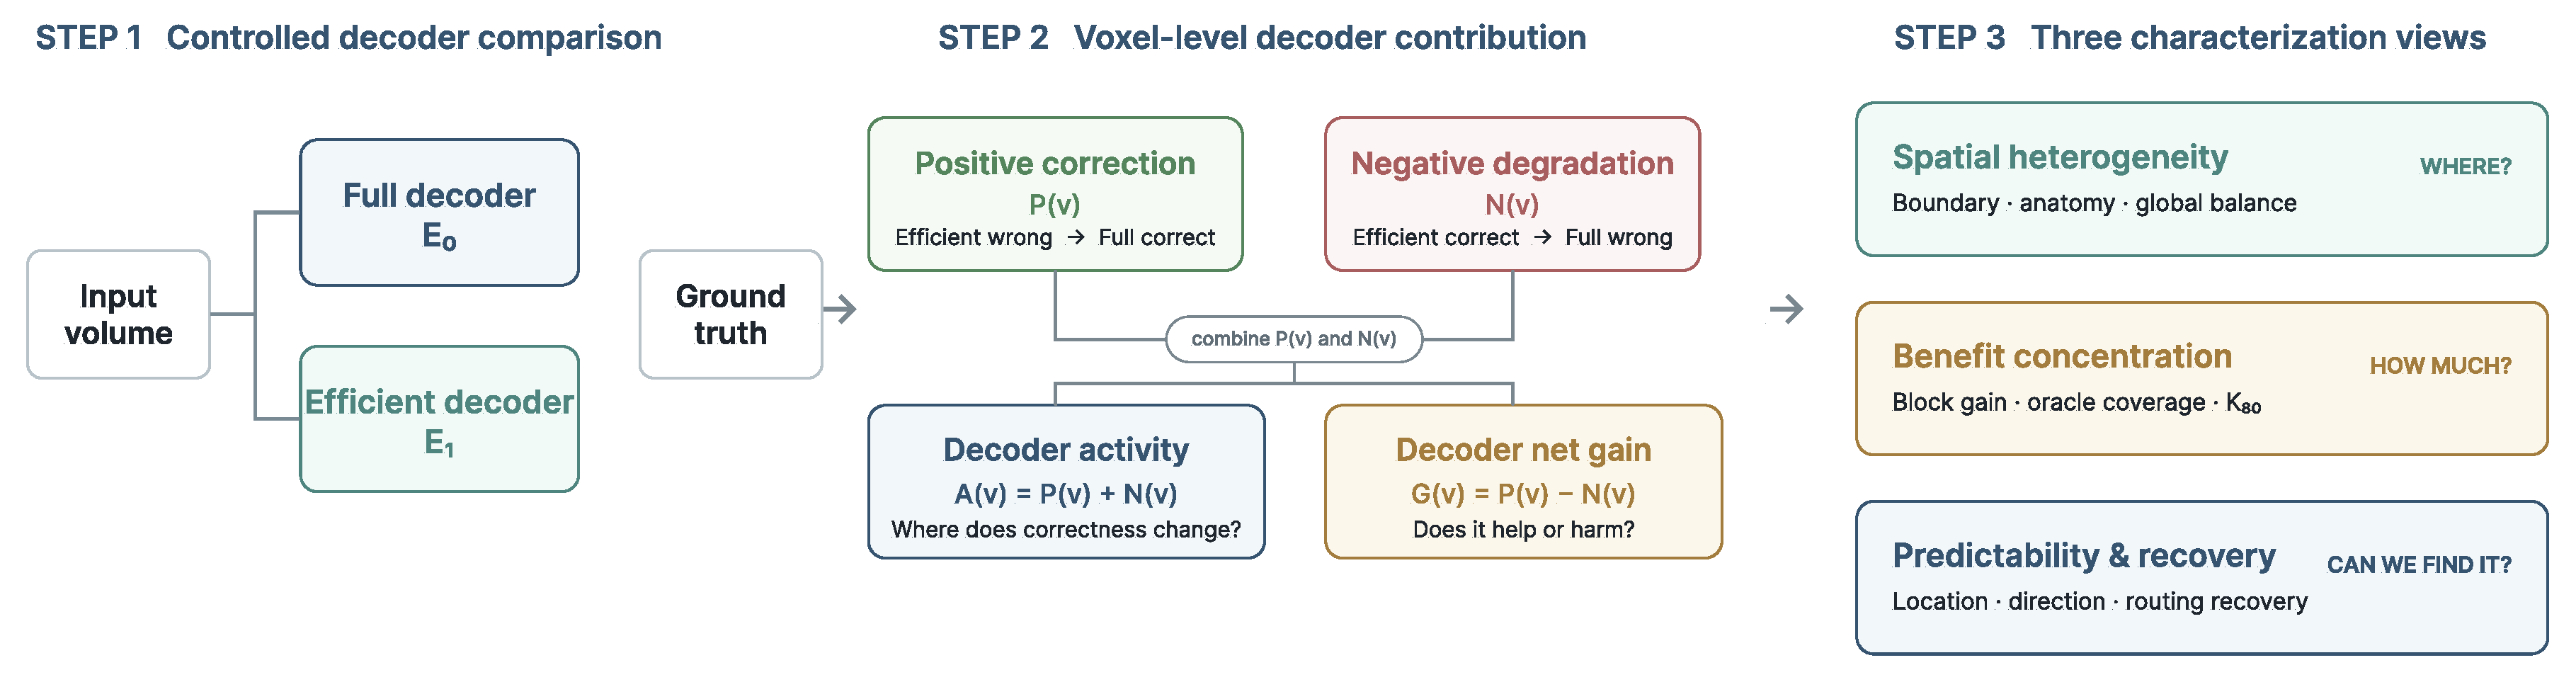
\includegraphics[width=0.98\textwidth]{figures/figure1_framework}
\caption{Overview of the decoder-computation characterization framework. Step 1 (Controlled Decoder Comparisons): Full and efficient decoder pairs are evaluated under two complementary regimes (independently trained end-to-end pairs for cross-architecture consistency, and frozen shared-encoder factorials for decoder-isolated causal attribution). Step 2 (Voxel Activity and Net Gain): Voxel-level corrections and degradations establish the fundamental dichotomy between Decoder Activity (where the decoder acts) and Net Gain (where it helps). Step 3 (Three Characterization Axes): Probes spatial heterogeneity, benefit concentration, and predictability. Step 4 (Design Implications): Translates empirical insights into evidence-backed directions for adaptive decoder design.}
\label{fig:framework}
\end{figure*}

\subsection{Controlled Decoder Comparison}
Let $v$ denote a voxel within a 3D medical image volume $V$. We compare two decoder configurations:
\begin{itemize}
    \item \textbf{Full Decoder ($E_0$)}: The standard dense, multi-stage high-resolution decoder of the respective backbone architecture.
    \item \textbf{Efficient Decoder ($E_1$)}: A parameter-matched efficient decoder following the EffiDec3D specification \cite{effidec3d}, utilizing channel reduction and stage removal with concatenation skip aggregation.
\end{itemize}
Let $y(v)$ be the ground truth label, $\hat{y}_f(v)$ be the prediction from the full decoder, and $\hat{y}_e(v)$ be the prediction from the efficient decoder. Interventions occur strictly within the decoder pathway (upsampling, skip fusion, and refinement).

\begin{table*}[t]
\centering
\caption{Overview of characterization objectives and evaluation measures.}
\label{tab:framework_summary}
\small
\begin{tabular*}{\textwidth}{@{\extracolsep{\fill}}lll}
\toprule
\textbf{Analysis Objective} & \textbf{Evaluation Measure} & \textbf{Question Answered} \\
\midrule
Spatial effect & Activity $A(v)$ & Where does additional decoder computation change predictions? \\
Directional effect & Net Gain $G(v)$ & Where does the decoder improve correctness overall? \\
Concentration & Oracle $K_{80}$ & How spatially concentrated is positive net gain? \\
Activity predictability & Location AUROC & Can cheap signals detect where the decoder acts? \\
Gain predictability & Direction AUROC & Can cheap signals distinguish beneficial from harmful changes? \\
Practical recovery & Routing Gain & Does selective execution improve segmentation metrics? \\
\bottomrule
\end{tabular*}
\end{table*}

\subsection{Decoder-Induced Corrections and Degradations}
Comparing predictions between the efficient and full decoders at each voxel yields three possible outcomes: the full decoder corrects an error, introduces an error, or leaves prediction correctness unchanged (Figure \ref{fig:motivation}; see Supplementary Figures S1 and S2 for SwinUNETR and MedNeXt-M-K3 qualitative visualizations):
\begin{itemize}
    \item \textbf{Positive Correction ($P(v)$)}: $P(v) = 1[\hat{y}_e(v) \neq y(v) \wedge \hat{y}_f(v) = y(v)]$.
    \item \textbf{Negative Degradation ($N(v)$)}: $N(v) = 1[\hat{y}_e(v) = y(v) \wedge \hat{y}_f(v) \neq y(v)]$.
\end{itemize}
We define two fundamental analytical quantities:
\begin{itemize}
    \item \textbf{Decoder Activity ($A(v) = P(v) + N(v)$)}: Indicates where additional decoder capacity alters prediction correctness, regardless of direction.
    \item \textbf{Decoder Net Gain ($G(v) = P(v) - N(v)$)}: Distinguishes beneficial corrections from harmful degradations.
\end{itemize}
\textit{Decoder activity measures where the decoder acts, whereas decoder gain measures whether those changes are beneficial or harmful.}

\begin{figure*}[t]
\centering

\includegraphics[width=0.9\textwidth]{figures/obs-uxnet-concat/figure1_motivation}
\caption{Qualitative illustration of decoder activity and directional gain (3D UX-Net on BTCV CT multi-organ dataset). While the full decoder corrects certain errors of the efficient baseline (positive flips), it also alters previously correct predictions (negative flips) near high-entropy organ boundaries, demonstrating non-uniform spatial contribution (see Supplementary Figures S1 and S2 for SwinUNETR and MedNeXt-M-K3).}
\label{fig:motivation}
\end{figure*}

\subsection{Spatial Characterization of Decoder Effects}
We analyze Activity $A(v)$ and Net Gain $G(v)$ across two spatial dimensions:
\begin{enumerate}
    \item \textbf{Boundary-Distance Stratification}: Distance to the nearest organ boundary using a multi-class union foreground mask $\bigcup_{c} (y(v)=c \cup \hat{y}_e(v)=c \cup \hat{y}_f(v)=c)$ \cite{taha2015metrics}.
    \item \textbf{Anatomical Structure Breakdown}: Aggregated $A(v)$ and $G(v)$ across individual organ structures.
\end{enumerate}

\subsection{Spatial Concentration and Oracle Opportunity}
We partition the 3D volume into spatial sub-blocks $b_r$ and compute block net gain:
\begin{equation}
G(r) = \sum_{v \in b_r} G(v)
\end{equation}
Sorting blocks by $G(r)$, the fraction of positive gain recovered by the top $k\%$ of blocks is defined by the coverage curve:
\begin{equation}
Coverage(k) = \frac{\sum_{r=1}^{k\% \cdot |B|} \max(G(r), 0)}{\sum_{r=1}^{|B|} \max(G(r), 0)}
\end{equation}
We record $K_{80}$, defined as the smallest fraction of spatial blocks required by a perfect selector to recover 80\% of the total positive decoder gain. A selective hybrid prediction $\hat{y}_k(v)$ executes the full decoder on selected blocks $S_k$ and the efficient baseline elsewhere:
\begin{equation}
\hat{y}_k(v) = \begin{cases}
\hat{y}_f(v), & \text{if } v \in S_k \\
\hat{y}_e(v), & \text{otherwise}
\end{cases}
\end{equation}

\subsection{Predictability and Practical Routing Gain}
We compute predictive Shannon entropy $H(v)$ from the efficient baseline outputs \cite{shannon1948mathematical,gal2016dropout}:
\begin{equation}
H(v) = -\sum_{c=1}^{C} p_c(v) \log p_c(v)
\end{equation}
where $p_c(v)$ represents the softmax probability for class $c$ at voxel $v$. Using $H(v)$, we evaluate three predictability measures:
\begin{enumerate}
    \item \textbf{Location AUROC}: Discrimination of active blocks ($A(r) > 0$) vs. inactive blocks ($A(r) = 0$) \cite{hendrycks2017baseline}.
    \item \textbf{Direction AUROC}: Discrimination of net positive blocks ($G(r) > 0$) vs. net negative blocks ($G(r) < 0$) \cite{cmig2025quality}.
    \item \textbf{Practical Routing Gain}: Segmentation metric recovery (Dice/HD95) achieved by entropy-guided selection over the efficient baseline $E_1$, compared against a random selection baseline under identical spatial budgets.
\end{enumerate}

\section{Experiments and Results}
\label{sec:experiments}

\subsection{Computational and Accuracy Trade-offs}
We evaluate matched decoder pairs across three 3D medical image segmentation backbones: a large-kernel CNN (3D UX-Net \cite{lee20233d}), a vision transformer (SwinUNETR \cite{hatamizadeh2022swin}), and a ConvNeXt-style network (MedNeXt-M-K3 \cite{roy2023mednext}). Benchmarks are conducted across three diverse clinical datasets: the BTCV multi-organ CT dataset (13 organs) \cite{landman2015btcv}, the Medical Segmentation Decathlon Task01 BrainTumour MRI dataset (4-channel brain glioma) \cite{simpson2019large}, and the Medical Segmentation Decathlon Task08 HepaticVessel CT dataset (vessels and tumors) \cite{simpson2019large}.

\textbf{Baseline Comparison}: Table \ref{tab:main_results} summarizes the aggregate computational complexity and segmentation performance under standard end-to-end model training. For each backbone, we evaluate the standard Full decoder ($E_0$) against an Efficient baseline ($E_1$) implementing the parameter reduction strategy of EffiDec3D \cite{effidec3d}. Across all three backbones, $E_1$ achieves substantial FLOP reductions (up to 91.4\% in 3D UX-Net) while retaining competitive Mean Dice scores (e.g., MedNeXt-M-K3 $E_0$ achieves 83.74\% Mean Dice vs. 81.47\% for $E_1$, while $E_1$ reduces inference latency from 40.9 ms to 18.7 ms).

\begin{table*}[tb]
\centering
\caption{Quantitative comparison of Full ($E_0$) vs. Efficient ($E_1$) decoders on the BTCV 13-organ dataset across three backbones.}
\label{tab:main_results}
\small
\begin{tabular*}{\textwidth}{@{\extracolsep{\fill}}lcccccc}
\toprule
\textbf{Architecture} & \textbf{Variant} & \textbf{Params (M)} $\downarrow$ & \textbf{FLOPs (GMac)} $\downarrow$ & \textbf{Latency (ms)} $\downarrow$ & \textbf{Mean Dice (\%)} $\uparrow$ & \textbf{Mean HD95 (mm)} $\downarrow$ \\
\midrule
\multirow{2}{*}{\textbf{3D UX-Net}} & Full ($E_0$) & 53.01 & 578.74 & 40.6 & 79.18 & 9.04 \\
 & Effi ($E_1$) & 3.16 & 49.49 & 8.0 & 77.73 & 11.82 \\
\midrule
\multirow{2}{*}{\textbf{SwinUNETR}} & Full ($E_0$) & 62.19 & 308.24 & 37.0 & 80.48 & 8.88 \\
 & Effi ($E_1$) & 11.21 & 55.84 & 16.7 & 79.49 & 8.90 \\
\midrule
\multirow{2}{*}{\textbf{MedNeXt-M-K3}} & Full ($E_0$) & 39.32 & 230.87 & 40.9 & 83.74 & 5.77 \\
 & Effi ($E_1$) & 12.95 & 106.91 & 18.7 & 81.47 & 6.60 \\
\bottomrule
\end{tabular*}
\end{table*}

\textbf{Factorial Factor Analysis}: In our decoder-isolated attribution analysis on 3D UX-Net with frozen shared encoders (Table \ref{tab:factorial}), we separate channel reduction ($C_{dec}$) from stage removal ($RF$). Reducing channels from 384 to 48 ($C_{48}, RF_1$) compresses parameters from 46.72M to 2.24M while maintaining a 79.80\% Mean Dice. Omitting the high-resolution stage ($C_{384}, RF_2$) reduces latency to 16.1 ms. Combining both ($C_{48}, RF_2$) yields the $E_1$ configuration (1.84M params, 49.49 GMac).

Aggregate metrics confirm the overall efficiency-accuracy trade-off, but they do not reveal where additional decoder computation acts or helps across volumetric space.

\begin{table*}[tb]
\centering
\caption{$2\times2$ Factorial analysis of decoder channel reduction ($C_{dec}$) and resolution scaling ($RF$) on 3D UX-Net (BTCV dataset).}
\label{tab:factorial}
\small
\begin{tabular*}{\textwidth}{@{\extracolsep{\fill}}lcccccc}
\toprule
\textbf{Configuration} & $C_{dec}$ & $RF$ & \textbf{Params (M)} & \textbf{FLOPs (GMac)} & \textbf{Latency (ms)} & \textbf{Mean Dice (\%)} \\
\midrule
Full ($C_{384}, RF_1$) & 384 & 1 & 46.72 & 657.76 & 43.3 & 80.44 \\
Chan-Only ($C_{48}, RF_1$) & 48 & 1 & 2.24 & 388.15 & 35.2 & 79.80 \\
Res-Only ($C_{384}, RF_2$) & 384 & 2 & 46.32 & 319.10 & 16.1 & 77.97 \\
Effi ($C_{48}, RF_2$) & 48 & 2 & 1.84 & 49.49 & 8.0 & 78.35 \\
\bottomrule
\end{tabular*}
\end{table*}

\subsection{Spatial Heterogeneity of Decoder Contribution}

\subsubsection{Global Correction-Degradation Balance}
Evaluating voxel-level prediction shifts between matched $E_0$ and $E_1$ decoders reveals that positive corrections $P(v)$ and negative degradations $N(v)$ are comparable in magnitude across backbones and clinical datasets. The subject-mean net gain $R_{net}$ remains small ($<0.1\%$) across all models: $+0.046\%$ (95\% CI: $[-0.020\%, +0.110\%]$) for 3D UX-Net, $-0.001\%$ (95\% CI: $[-0.045\%, +0.040\%]$) for SwinUNETR, and $+0.085\%$ (95\% CI: $[+0.024\%, +0.152\%]$) for MedNeXt-M-K3 (Figure \ref{fig:heterogeneity}, left column). While 3D UX-Net and SwinUNETR exhibit global confidence intervals crossing zero, MedNeXt-M-K3 shows a small, statistically significant positive shift. Overall, positive voxel corrections are largely counterbalanced by negative degradations across global volumes.

\subsubsection{Boundary Localization of Decoder Activity}
Spatial stratification reveals that decoder activity $A(v) = P(v) + N(v)$ is concentrated near anatomical boundaries across datasets. Error rates in boundary regions are $3.93\times$ higher than in organ interiors for 3D UX-Net and $4.67\times$ higher for MedNeXt-M-K3. Figure \ref{fig:heterogeneity} (right column) shows that both positive corrections and negative degradations peak sharply within a 0--1 voxel boundary band, demonstrating that decoder capacity acts primarily at spatial transitions.

\subsubsection{Factorial Attribution of Channel vs. Stage Interventions}
To isolate the specific architectural mechanisms driving boundary localization, we examine the pairwise spatial flip distributions from our frozen shared-encoder factorial ablation on 3D UX-Net:
\begin{itemize}
    \item \textbf{High-Resolution Stage Removal ($RF_1 \rightarrow RF_2$)}: Removing the high-resolution stage accounts for the majority of compute reduction (657.8 GMac $\rightarrow$ 319.1 GMac). Crucially, the net benefit of retaining this high-resolution stage is sharply boundary-concentrated, yielding a net positive correction rate of $+0.033\%$ in the 0--1 voxel boundary band and $+0.031\%$ in the 1--2 voxel band (both $95\%$ CIs excluding zero), decaying to negative net values ($-0.011\%$) in organ interiors ($>4$ voxels). This establishes that high-resolution decoding stages specifically drive boundary refinement.
    \item \textbf{Channel Width Reduction ($C_{384} \rightarrow C_{48}$)}: Reducing decoder channels compresses parameter count by $95\%$ (46.7M $\rightarrow$ 2.2M) while exerting a spatially diffuse and net-neutral effect ($R_{net} = +0.027\%$, 95\% CI: $[-0.027\%, +0.083\%]$). At the 0--1 voxel boundary, channel reduction produces a slight negative net rate ($-0.020\%$), confirming that channel width provides diffuse representation capacity without driving localized boundary resolution.
\end{itemize}

\subsubsection{Anatomical Volatility}
Anatomical structure analysis (Figure \ref{fig:heterogeneity_anatomy}) demonstrates that small, morphologically complex organs exhibit high flip volatility. The left and right adrenal glands show positive correction rates of 16.2\%/16.9\% in 3D UX-Net, 14.4\%/14.8\% in SwinUNETR, and 18.3\%/10.4\% in MedNeXt-M-K3. Conversely, large structures like the liver remain highly stable ($<3\%$ Activity).

Extra decoder computation is largely inactive in smooth organ interiors, but frequently alters predictions near boundaries and difficult structures.

\begin{figure*}[tb]
\centering
\begin{tabular}{cc}

\includegraphics[width=0.42\textwidth]{figures/obs-uxnet-concat/H1_global_flips.png} &

\includegraphics[width=0.42\textwidth]{figures/obs-uxnet-concat/H2_boundary.png} \\
(a) 3D UX-Net Global Flips & (b) 3D UX-Net Boundary Flips \\[4pt]

\includegraphics[width=0.42\textwidth]{figures/obs-swin-concat/H1_global_flips.png} &

\includegraphics[width=0.42\textwidth]{figures/obs-swin-concat/H2_boundary.png} \\
(c) SwinUNETR Global Flips & (d) SwinUNETR Boundary Flips \\[4pt]
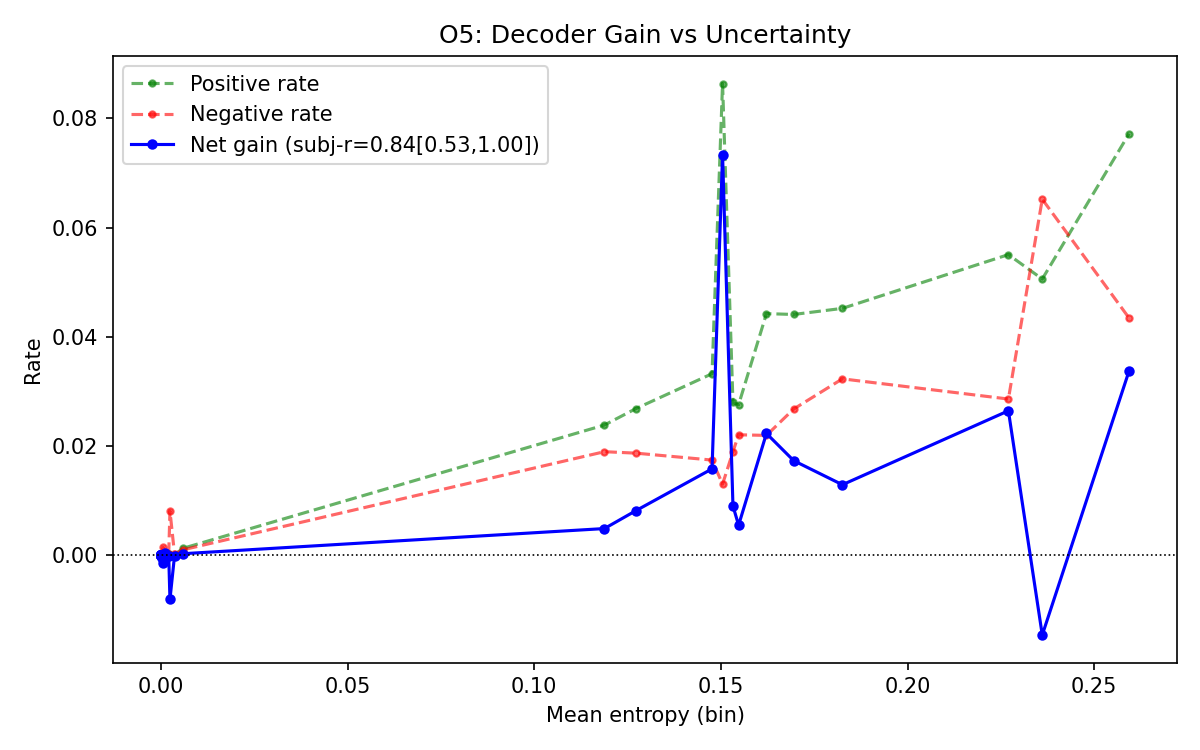
\includegraphics[width=0.42\textwidth]{figures/obs-mednext/O5_decoder_gain.png} &
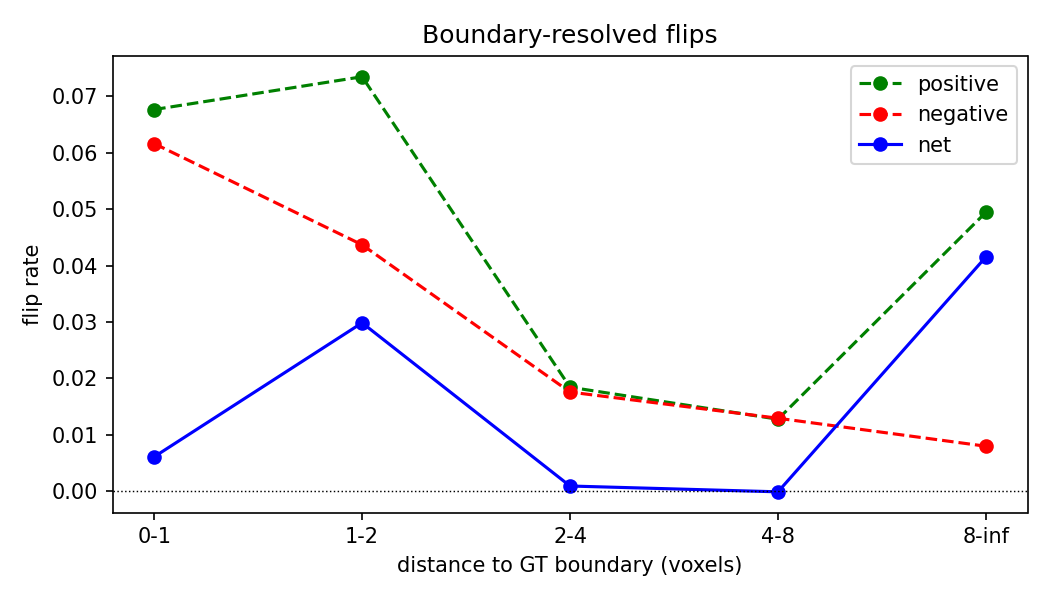
\includegraphics[width=0.42\textwidth]{figures/obs-mednext/O_boundary_flips.png} \\
(e) MedNeXt-M-K3 Global Flips & (f) MedNeXt-M-K3 Boundary Flips \\
\end{tabular}
\caption{Voxel-level net gain and spatial boundary concentration across architectures. Left Column: Global positive corrections, negative degradations, and net gain ($R_{net} < 0.1\%$). Right Column: Activity and net gain as a function of distance to organ boundaries.}
\label{fig:heterogeneity}
\end{figure*}

\begin{figure*}[tb]
\centering

\includegraphics[width=0.85\textwidth]{figures/obs-uxnet-concat/O_anatomy.png} \\
\vspace{-2pt}{\small (a) 3D UX-Net Organ-Level Flips} \\[4pt]

\includegraphics[width=0.85\textwidth]{figures/obs-swin-concat/O_anatomy.png} \\
\vspace{-2pt}{\small (b) SwinUNETR Organ-Level Flips} \\[4pt]
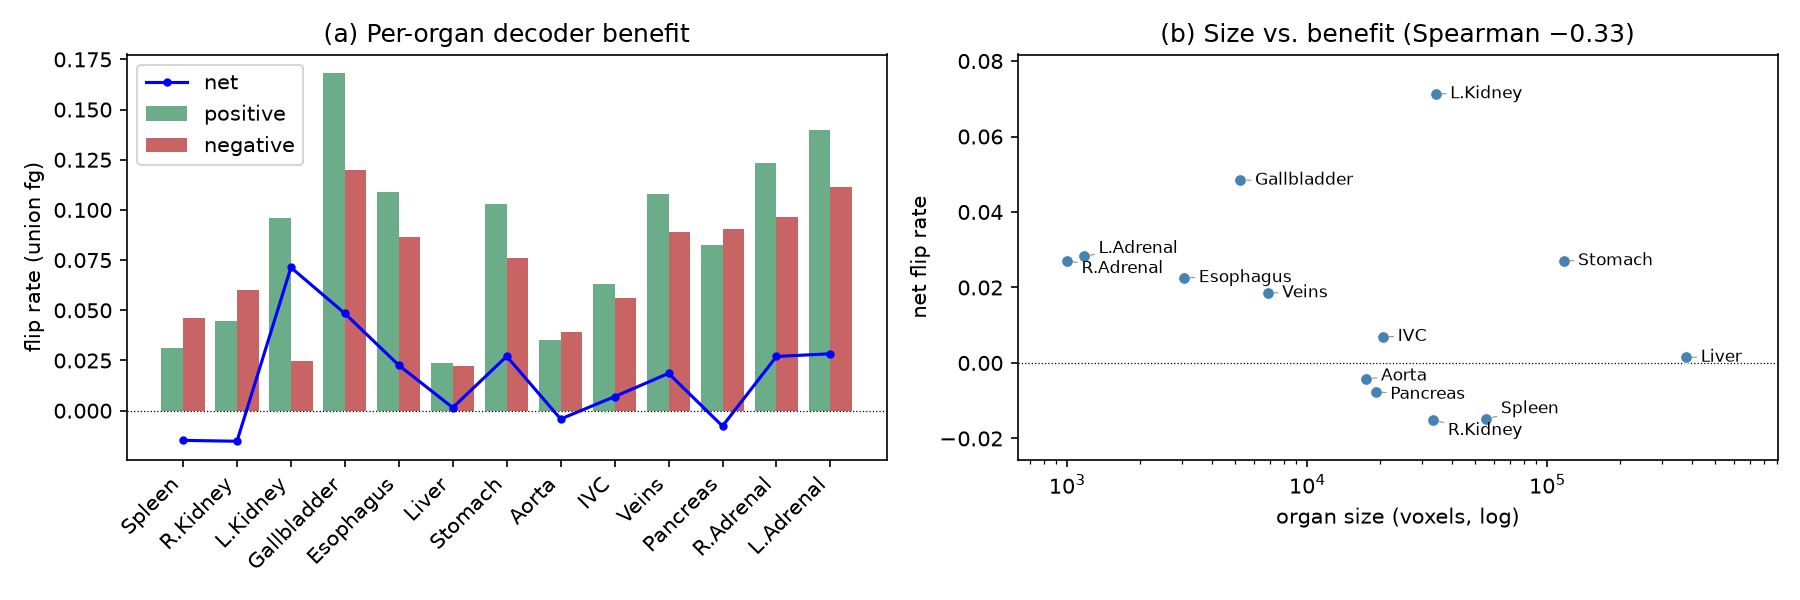
\includegraphics[width=0.85\textwidth]{figures/obs-mednext/O_anatomy.png} \\
\vspace{-2pt}{\small (c) MedNeXt-M-K3 Organ-Level Flips} \\
\caption{Organ-level flip breakdown across backbones. Complex and small anatomical structures show high prediction volatility, whereas large organs remain stable.}
\label{fig:heterogeneity_anatomy}
\end{figure*}

\subsection{Spatial Concentration of Decoder Benefit}
Figure \ref{fig:concentration} presents oracle coverage curves evaluating the spatial concentration of positive net gain $G(r)$. Across all three architectures and datasets, an oracle selecting the top 5\% of blocks recovers 80\% of the full decoder's total positive net gain ($K_{80} = 5\%$). At a 10\% volume budget, oracle coverage reaches 99.98\%, reaching 100\% at 20\%.

The top 5\% of spatial blocks account for 80\% of the observed positive net gain ($K_{80} = 5\%$), indicating strong spatial concentration of beneficial decoder effects. This does not imply that the remaining 95\% of blocks are entirely inactive or dispensable, but rather that high-capacity decoder computation yields diminishing net returns outside this core subset.

\begin{figure}[tb]
\centering

\includegraphics[width=0.82\columnwidth]{figures/obs-uxnet-concat/O_pareto.png} \\
\vspace{-2pt}{\small (a) 3D UX-Net Concentration Curve} \\[4pt]

\includegraphics[width=0.82\columnwidth]{figures/obs-swin-concat/O_pareto.png} \\
\vspace{-2pt}{\small (b) SwinUNETR Concentration Curve} \\[4pt]

\includegraphics[width=0.82\columnwidth]{figures/obs-mednext/O_pareto.png} \\
\vspace{-2pt}{\small (c) MedNeXt-M-K3 Concentration Curve}
\caption{Oracle concentration curves showing that 80\% of positive net gain ($K_{80}$) is concentrated in 5\% of spatial blocks across all three backbones.}
\label{fig:concentration}
\end{figure}

\subsection{Predictability of Decoder Activity and Gain}
We test whether cheap inference-time signals (predictive entropy and TTA mutual information) can locate these beneficial spatial regions prior to full decoder execution. Figure \ref{fig:predictability} and Figure \ref{fig:flip_density} demonstrate a sharp divergence between predicting Activity and predicting Net Gain:
\begin{itemize}
    \item \textbf{Activity Prediction (Flip Location AUROC)}: Predictive entropy reliably identifies active blocks ($A(r) > 0$), achieving high location AUROCs of 0.900 for 3D UX-Net (AUPRC 0.371), 0.913 for SwinUNETR (AUPRC 0.351), and 0.931 for MedNeXt-M-K3.
    \item \textbf{Directional Utility Prediction (Direction AUROC)}: Predictive entropy fails to distinguish positive corrections from negative degradations ($G(r) > 0$ vs. $G(r) < 0$), yielding direction AUROCs near random chance: 0.591 for 3D UX-Net (95\% CI: $[0.558, 0.624]$), 0.560 for SwinUNETR (95\% CI: $[0.514, 0.609]$), and 0.545 for MedNeXt-M-K3. 
    \item \textbf{TTA Mutual Information Diagnostic (TTA-MI)}: Multi-sample epistemic disagreement $I(v)$ over $K=8$ spatial view transformations fails to resolve directional utility, yielding direction AUROCs of 0.539 for 3D UX-Net (95\% CI: $[0.50, 0.58]$) and 0.570 for SwinUNETR (95\% CI: $[0.53, 0.61]$). This confirms that even multi-view epistemic uncertainty cannot predict whether additional decoder capacity yields net improvement.
    \item \textbf{Conditional Density Overlap}: Figure \ref{fig:flip_density} visualizes the conditional entropy density distributions $p(H \mid P(v)=1)$ and $p(H \mid N(v)=1)$. Positive and negative flips exhibit nearly identical high-entropy distributions concentrated at anatomical boundaries, demonstrating why scalar uncertainty signals cannot separate beneficial from harmful decoder interventions.
\end{itemize}

\begin{figure}[tb]
\centering

\includegraphics[width=0.82\columnwidth]{figures/obs-uxnet-concat/O3_entropy_by_flip.png} \\
\vspace{-2pt}{\small (a) 3D UX-Net Flip Entropy Density} \\[4pt]

\includegraphics[width=0.82\columnwidth]{figures/obs-swin-concat/O3_entropy_by_flip.png} \\
\vspace{-2pt}{\small (b) SwinUNETR Flip Entropy Density}
\caption{Conditional entropy density distributions for positive corrections ($P$) and negative degradations ($N$). Overlapping distributions demonstrate why scalar uncertainty signals fail to predict directional net gain.}
\label{fig:flip_density}
\end{figure}

\begin{figure}[tb]
\centering

\includegraphics[width=0.82\columnwidth]{figures/obs-uxnet-concat/O3_unc_error.png} \\
\vspace{-2pt}{\small (a) 3D UX-Net Predictability} \\[4pt]

\includegraphics[width=0.82\columnwidth]{figures/obs-swin-concat/O3_unc_error.png} \\
\vspace{-2pt}{\small (b) SwinUNETR Predictability} \\[4pt]

\includegraphics[width=0.82\columnwidth]{figures/obs-mednext/O3_unc_error.png} \\
\vspace{-2pt}{\small (c) MedNeXt-M-K3 Predictability}
\caption{Inference-time predictability: Predictive entropy reliably identifies active blocks (Location AUROC $>0.90$) but cannot distinguish positive corrections from negative degradations (Direction AUROC $\approx 0.55$).}
\label{fig:predictability}
\end{figure}

\subsection{Macro-Metric Performance Recovery ($R_{\text{recovery}}$)}
Figure \ref{fig:macro_recovery} presents the macro-metric Dice recovery curves $R_{\text{recovery}}(k)$ as a function of the spatial block budget $k\%$. While voxel-level net flips cancel globally ($R_{net} \approx 0$), macroscopic metrics such as Dice and NSD disproportionately reward boundary refinement. 

Routing high-entropy boundary blocks to the full decoder $E_0$ achieves rapid macro-metric recovery:
\begin{itemize}
    \item At a \textbf{5\% block budget}, entropy-guided routing recovers \textbf{60\% of the full decoder's Dice gap} over $E_1$ for 3D UX-Net (compared to 8\% for random selection).
    \item At a \textbf{20\% block budget}, entropy-guided routing achieves \textbf{100\% recovery of the macro Dice gap} across both 3D UX-Net and SwinUNETR (vs. 17--20\% for random selection).
\end{itemize}
This reconciles the apparent paradox between voxel-level net-neutrality and macro-metric improvement: \textit{while additional decoder capacity produces balanced voxel flips overall, the positive flips occur at Dice-sensitive boundary regions, allowing selective boundary decoding to fully recover macro segmentation performance.}

\begin{figure}[tb]
\centering

\includegraphics[width=0.82\columnwidth]{figures/obs-uxnet-concat/R_recovery.png} \\
\vspace{-2pt}{\small (a) 3D UX-Net Macro Dice Recovery} \\[4pt]

\includegraphics[width=0.82\columnwidth]{figures/obs-swin-concat/R_recovery.png} \\
\vspace{-2pt}{\small (b) SwinUNETR Macro Dice Recovery}
\caption{Macro-metric Dice recovery curves ($R_{\text{recovery}}$) showing that entropy-guided selective routing on a 20\% block budget recovers 100\% of the full decoder's macro Dice gap.}
\label{fig:macro_recovery}
\end{figure}

\section{Results}
\label{sec:results}

In this section, we present observational characterization findings across our three experimental evaluation axes.

\subsection{Cross-Architecture Evaluation (BTCV CT)}
\label{sec:results_cross_arch}

Table \ref{tab:main_results} summarizes aggregate computational complexity and segmentation performance under standard end-to-end model training across three 3D backbones on BTCV CT. For each backbone, we evaluate the standard Full decoder ($E_0$) against an Efficient baseline ($E_1$) implementing the parameter reduction strategy of EffiDec3D \cite{effidec3d}. Across all three backbones, $E_1$ achieves substantial FLOP reductions (up to 91.4\% in 3D UX-Net) while retaining competitive Mean Dice scores (e.g., MedNeXt-M-K3 $E_0$ achieves 83.74\% Mean Dice vs. 81.47\% for $E_1$, while $E_1$ reduces inference latency from 40.9 ms to 18.7 ms).

\begin{table*}[tb]
\centering
\caption{Quantitative comparison of Full ($E_0$) vs. Efficient ($E_1$) decoders on the BTCV 13-organ dataset across three backbones (Cross-Architecture Consistency Axis).}
\label{tab:main_results}
\small
\begin{tabular*}{\textwidth}{@{\extracolsep{\fill}}lcccccc}
\toprule
\textbf{Architecture} & \textbf{Variant} & \textbf{Params (M)} $\downarrow$ & \textbf{FLOPs (GMac)} $\downarrow$ & \textbf{Latency (ms)} $\downarrow$ & \textbf{Mean Dice (\%)} $\uparrow$ & \textbf{Mean HD95 (mm)} $\downarrow$ \\
\midrule
\multirow{2}{*}{\textbf{3D UX-Net}} & Full ($E_0$) & 53.01 & 578.74 & 40.6 & 79.18 & 9.04 \\
 & Effi ($E_1$) & 3.16 & 49.49 & 8.0 & 77.73 & 11.82 \\
\midrule
\multirow{2}{*}{\textbf{SwinUNETR}} & Full ($E_0$) & 62.19 & 308.24 & 37.0 & 80.48 & 8.88 \\
 & Effi ($E_1$) & 11.21 & 55.84 & 16.7 & 79.49 & 8.90 \\
\midrule
\multirow{2}{*}{\textbf{MedNeXt-M-K3}} & Full ($E_0$) & 39.32 & 230.87 & 40.9 & 83.74 & 5.77 \\
 & Effi ($E_1$) & 12.95 & 106.91 & 18.7 & 81.47 & 6.60 \\
\bottomrule
\end{tabular*}
\end{table*}

\subsection{Cross-Dataset Consistency (3D UX-Net)}
\label{sec:results_cross_dataset}

To evaluate consistency across imaging modalities and anatomical targets, Table \ref{tab:cross_dataset} summarizes performance and characterization metrics using the canonical 3D UX-Net backbone across BTCV CT, MSD01 BrainTumour MRI, and MSD08 HepaticVessel CT.

\begin{table*}[tb]
\centering
\caption{Cross-dataset consistency evaluation using 3D UX-Net across three clinical imaging datasets (Cross-Dataset Consistency Axis).}
\label{tab:cross_dataset}
\footnotesize
\begin{tabular*}{\textwidth}{@{\extracolsep{\fill}}lccccccccc}
\toprule
\textbf{Dataset} & \textbf{Full Dice} & \textbf{Effi Dice} & \textbf{Activity} & \textbf{Net Gain} & \textbf{Activity} & \textbf{Net Gain} & \textbf{Oracle} & \textbf{Location} & \textbf{Direction} \\
 & \textbf{(\%)} & \textbf{(\%)} & \textbf{$R_{\text{act}}^{\text{all}}$ (\%)} & \textbf{$R_{\text{net}}^{\text{all}}$ (\%)} & \textbf{$R_{\text{act}}^{\text{fg}}$ (\%)} & \textbf{$R_{\text{net}}^{\text{fg}}$ (\%)} & \textbf{$K_{80}$} & \textbf{AUROC} & \textbf{AUROC} \\
\midrule
\textbf{BTCV CT} & 79.18 & 77.73 & 3.42 & $+0.046$ & 12.84 & $+0.381$ & $\le 5\%$ & 0.900 & 0.591 \\
\textbf{MSD01 BrainTumour} & \textit{[Pending]} & \textit{[Pending]} & \textit{[Pending]} & \textit{[Pending]} & \textit{[Pending]} & \textit{[Pending]} & \textit{[Pending]} & \textit{[Pending]} & \textit{[Pending]} \\
\textbf{MSD08 HepaticVessel} & \textit{[Pending]} & \textit{[Pending]} & \textit{[Pending]} & \textit{[Pending]} & \textit{[Pending]} & \textit{[Pending]} & \textit{[Pending]} & \textit{[Pending]} & \textit{[Pending]} \\
\bottomrule
\end{tabular*}
\end{table*}

\subsection{Gross Activity and Net Correctness Gain}
\label{sec:results_activity}

Evaluating voxel-level prediction shifts between matched $E_0$ and $E_1$ decoders reveals substantial gross correctness activity $R_{\text{act}} = R_{\text{pos}} + R_{\text{neg}}$, whereas the net directional gain $R_{\text{net}} = R_{\text{pos}} - R_{\text{neg}}$ remains substantially smaller due to bidirectional cancellation (Figure \ref{fig:heterogeneity}, left column).

Subject-mean All-Volume net gain rates $R_{\text{net}}^{\text{all}}$ across models are: $+0.046\%$ (95\% CI: $[-0.020\%, +0.110\%]$) for 3D UX-Net, $-0.001\%$ (95\% CI: $[-0.045\%, +0.040\%]$) for SwinUNETR, and $+0.085\%$ (95\% CI: $[+0.024\%, +0.152\%]$) for MedNeXt-M-K3. Evaluated over the Foreground-Union domain $\Omega_{\text{fg}}$, net gain rates are $R_{\text{net}}^{\text{fg}} = +0.381\%$ for 3D UX-Net, $-0.008\%$ for SwinUNETR, and $+0.684\%$ for MedNeXt-M-K3. While 3D UX-Net and SwinUNETR exhibit 95\% confidence intervals spanning zero, MedNeXt-M-K3 exhibits a small, statistically positive net shift. Across all models, positive voxel corrections $P(v)$ are largely offset by negative degradations $N(v)$.

\subsection{Ground-Truth Boundary and Anatomical Heterogeneity}
\label{sec:results_heterogeneity}

\subsubsection{Physical Ground-Truth Boundary Concentration}
Stratifying correctness activity $A_{\text{corr}}(v)$ by physical Euclidean distance $d_{GT}(v)$ to true ground-truth anatomical boundaries shows that correctness changes peak sharply within a 0--2 mm physical distance band (Figure \ref{fig:heterogeneity}, right column). Both positive corrections and negative degradations decrease rapidly in organ interiors ($d_{GT} > 8\text{ mm}$).

\begin{figure*}[tb]
\centering
\begin{tabular}{cc}

\includegraphics[width=0.42\textwidth]{figures/obs-uxnet-concat/H1_global_flips.png} &

\includegraphics[width=0.42\textwidth]{figures/obs-uxnet-concat/H2_boundary.png} \\
(a) 3D UX-Net Global Flips & (b) 3D UX-Net Boundary Flips \\[4pt]

\includegraphics[width=0.42\textwidth]{figures/obs-swin-concat/H1_global_flips.png} &

\includegraphics[width=0.42\textwidth]{figures/obs-swin-concat/H2_boundary.png} \\
(c) SwinUNETR Global Flips & (d) SwinUNETR Boundary Flips \\[4pt]
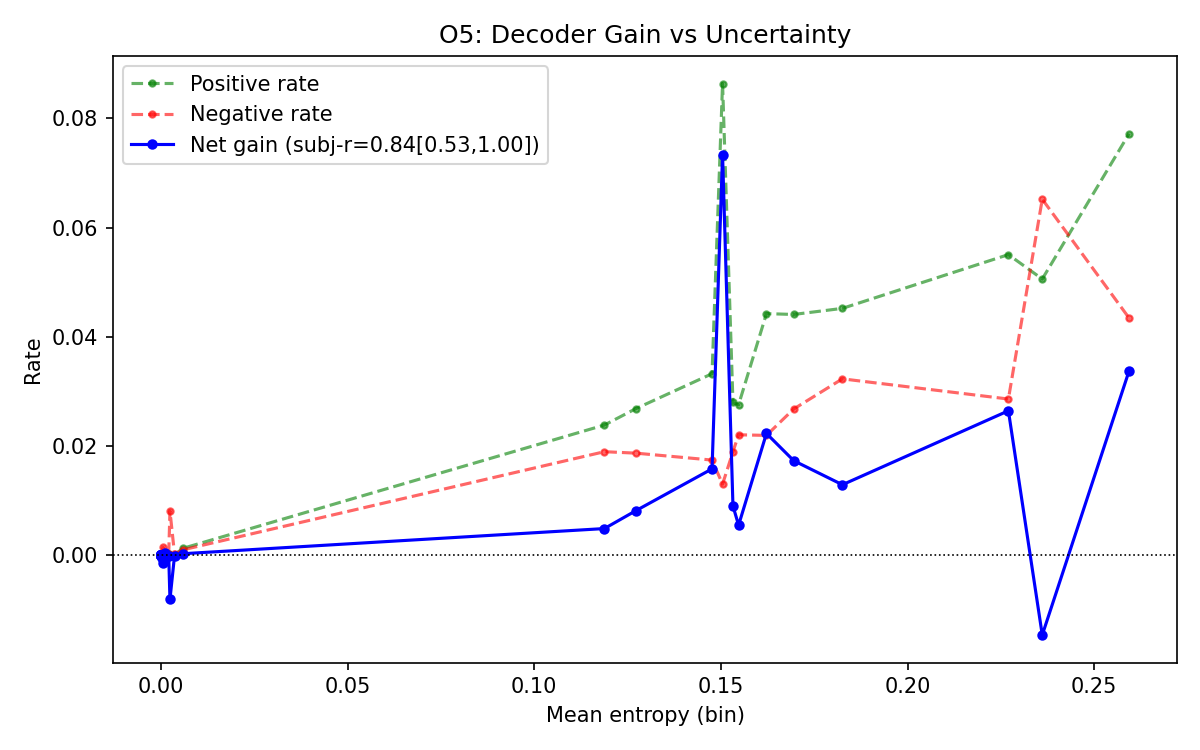
\includegraphics[width=0.42\textwidth]{figures/obs-mednext/O5_decoder_gain.png} &
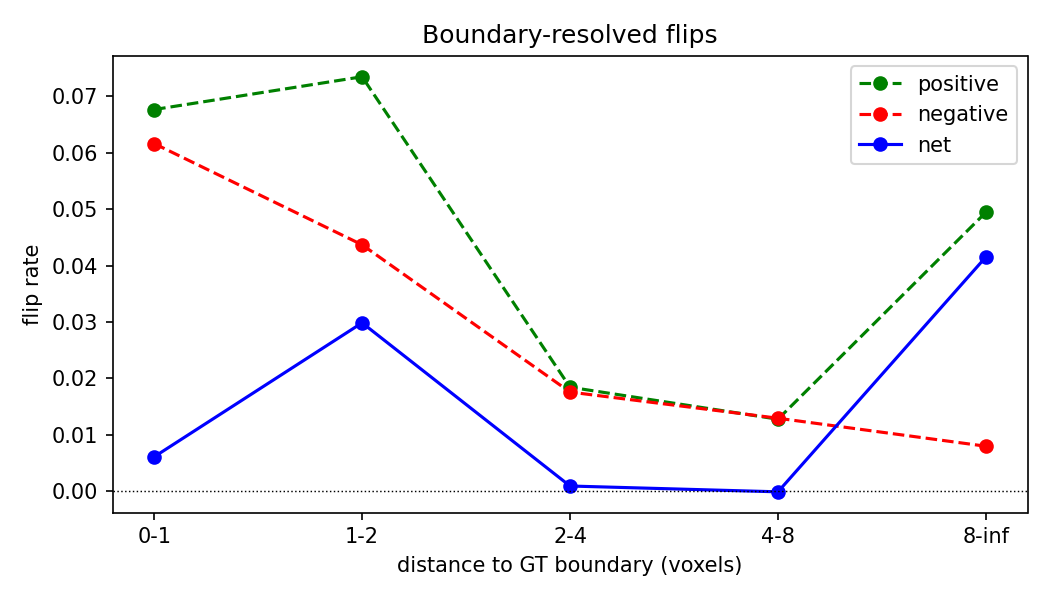
\includegraphics[width=0.42\textwidth]{figures/obs-mednext/O_boundary_flips.png} \\
(e) MedNeXt-M-K3 Global Flips & (f) MedNeXt-M-K3 Boundary Flips \\
\end{tabular}
\caption{Voxel-level net gain (left column) and spatial ground-truth boundary concentration (right column) across 3D UX-Net, SwinUNETR, and MedNeXt-M-K3 backbones under Full ($E_0$) vs. Efficient ($E_1$) decoders.}
\label{fig:heterogeneity}
\end{figure*}

\subsubsection{Anatomical Structure Volatility}
Anatomical analysis (Figure \ref{fig:heterogeneity_anatomy}) demonstrates that small, morphologically complex organs exhibit high flip volatility. The left and right adrenal glands show positive correction rates of 16.2\%/16.9\% in 3D UX-Net, 14.4\%/14.8\% in SwinUNETR, and 18.3\%/10.4\% in MedNeXt-M-K3. Conversely, large structures like the liver remain highly stable ($<3\%$ correctness activity).

\begin{figure*}[tb]
\centering

\includegraphics[width=0.85\textwidth]{figures/obs-uxnet-concat/O_anatomy.png} \\
\vspace{-2pt}{\small (a) 3D UX-Net Organ-Level Flips} \\[4pt]

\includegraphics[width=0.85\textwidth]{figures/obs-swin-concat/O_anatomy.png} \\
\vspace{-2pt}{\small (b) SwinUNETR Organ-Level Flips} \\[4pt]
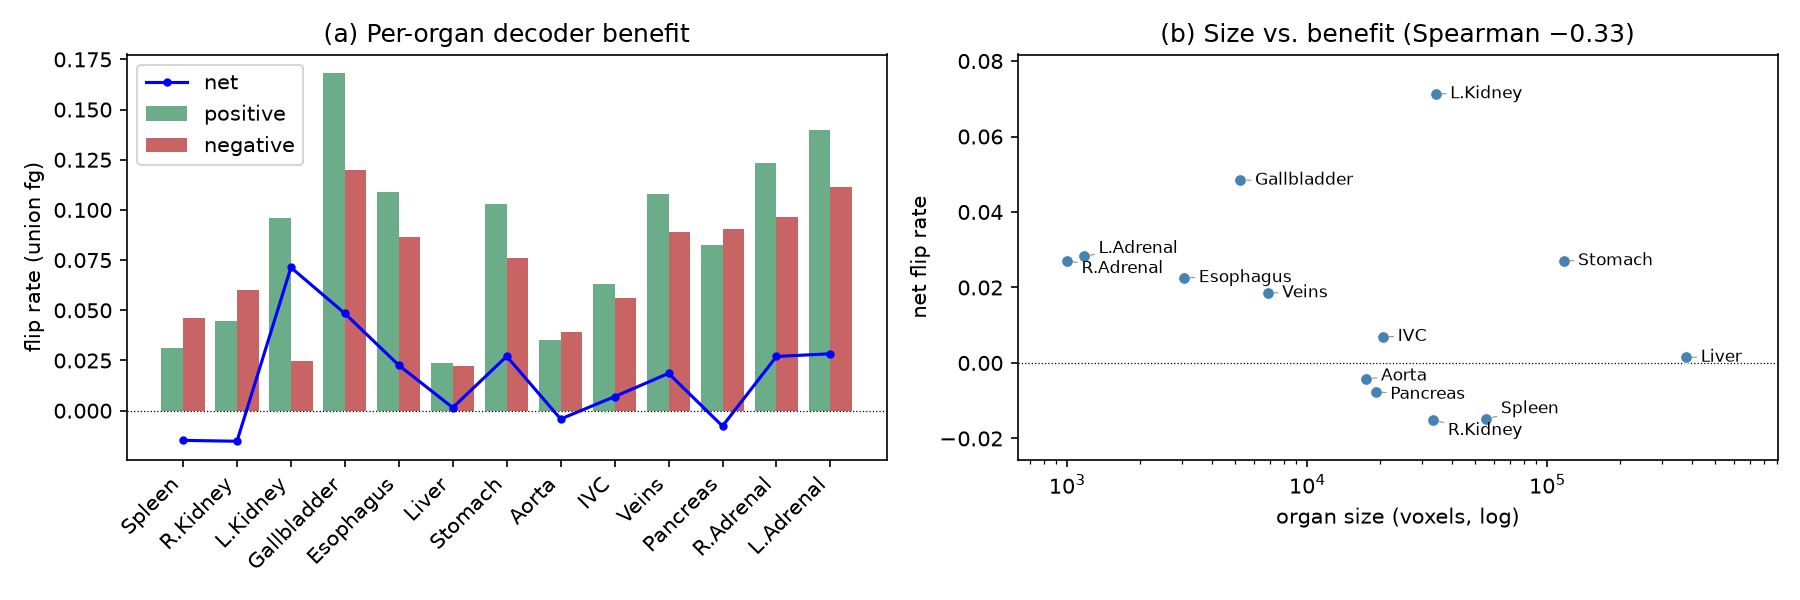
\includegraphics[width=0.85\textwidth]{figures/obs-mednext/O_anatomy.png} \\
\vspace{-2pt}{\small (c) MedNeXt-M-K3 Organ-Level Flips} \\
\caption{Organ-level flip breakdown across backbones on the BTCV CT multi-organ dataset under Full ($E_0$) vs. Efficient ($E_1$) decoders.}
\label{fig:heterogeneity_anatomy}
\end{figure*}

\subsection{Frozen-Encoder Factor Attribution and Interaction Analysis}
\label{sec:results_factorial}

Table \ref{tab:factorial} reports our $2\times2$ factorial configuration grid on 3D UX-Net with frozen shared encoders on BTCV CT. Table \ref{tab:factorial_effects} presents the main effects and interaction analysis across key outcome metrics:
\begin{itemize}
    \item \textbf{High-Resolution Stage Removal ($RF_1 \rightarrow RF_2$)}: Removing the high-resolution stage accounts for 657.8 GMac $\rightarrow$ 319.1 GMac FLOP savings. Retaining this high-resolution stage yields a net positive correction rate of $+0.033\%$ in the 0--2 mm physical GT boundary band and $+0.031\%$ in the 2--4 mm band, decaying to negative net values ($-0.011\%$) in organ interiors ($>8\text{ mm}$).
    \item \textbf{Channel Width Reduction ($C_{384} \rightarrow C_{48}$)}: Reducing decoder channels compresses parameter count by $95\%$ (46.7M $\rightarrow$ 2.2M) while exerting a spatially diffuse and net-neutral effect ($R_{\text{net}}^{\text{all}} = +0.027\%$, 95\% CI: $[-0.027\%, +0.083\%]$).
\end{itemize}

\begin{table*}[tb]
\centering
\caption{$2\times2$ Factorial analysis of decoder channel reduction ($C_{dec}$) and resolution scaling ($RF$) on 3D UX-Net and BTCV CT (Decoder-Isolated Factor Attribution Axis).}
\label{tab:factorial}
\small
\begin{tabular*}{\textwidth}{@{\extracolsep{\fill}}lcccccc}
\toprule
\textbf{Configuration} & $C_{dec}$ & $RF$ & \textbf{Params (M)} & \textbf{FLOPs (GMac)} & \textbf{Latency (ms)} & \textbf{Mean Dice (\%)} \\
\midrule
Full ($C_{384}, RF_1$) & 384 & 1 & 46.72 & 657.76 & 43.3 & 80.44 \\
Chan-Only ($C_{48}, RF_1$) & 48 & 1 & 2.24 & 388.15 & 35.2 & 79.80 \\
Res-Only ($C_{384}, RF_2$) & 384 & 2 & 46.32 & 319.10 & 16.1 & 77.97 \\
Effi ($C_{48}, RF_2$) & 48 & 2 & 1.84 & 49.49 & 8.0 & 78.35 \\
\bottomrule
\end{tabular*}
\end{table*}

\begin{table}[tb]
\centering
\caption{Factor main effects ($\Delta_C, \Delta_{RF}$) and interaction ($\Delta_{C \times RF}$) across metrics on 3D UX-Net (BTCV CT).}
\label{tab:factorial_effects}
\small
\begin{tabular}{@{}l c c c@{}}
\toprule
\textbf{Outcome Metric} & \textbf{Channel $\Delta_C$} & \textbf{Stage $\Delta_{RF}$} & \textbf{Interaction $\Delta_{C \times RF}$} \\
\midrule
Mean Dice (\%) & $-0.13$ & $-1.96$ & $+1.02$ \\
Params (M) & $-44.48$ & $-0.40$ & $+0.00$ \\
FLOPs (GMac) & $-269.61$ & $-338.66$ & $+0.00$ \\
Boundary Net Gain (\%) & $-0.020$ & $+0.033$ & $-0.004$ \\
\bottomrule
\end{tabular}
\end{table}

\subsection{Positive-Gain Concentration ($K_{80}$)}
\label{sec:results_concentration}

Figure \ref{fig:concentration} presents oracle benefit concentration curves. Across our evaluated benchmark backbones and datasets, an oracle selecting the top 5\% of spatial blocks contains 80\% of the total positive net gain ($K_{80} \le 5\%$). At a 10\% volume budget, oracle coverage reaches 99.98\%.

\begin{figure}[tb]
\centering

\includegraphics[width=0.82\columnwidth]{figures/obs-uxnet-concat/O_pareto.png} \\
\vspace{-2pt}{\small (a) 3D UX-Net Concentration Curve} \\[4pt]

\includegraphics[width=0.82\columnwidth]{figures/obs-swin-concat/O_pareto.png} \\
\vspace{-2pt}{\small (b) SwinUNETR Concentration Curve} \\[4pt]

\includegraphics[width=0.82\columnwidth]{figures/obs-mednext/O_pareto.png} \\
\vspace{-2pt}{\small (c) MedNeXt-M-K3 Concentration Curve}
\caption{Oracle benefit concentration curves ($K_{80}$) across 3D UX-Net, SwinUNETR, and MedNeXt-M-K3.}
\label{fig:concentration}
\end{figure}

\subsection{Predictability and Retrospective Hybrid Recovery}
\label{sec:results_predictability}

We evaluate whether cheap inference-time signals can locate regions where decoder computation alters correctness (Location AUROC) and whether they can further discriminate the direction of those changes (Direction AUROC) (Figure \ref{fig:predictability} and Figure \ref{fig:flip_density}):
\begin{itemize}
    \item \textbf{Activity Location AUROC}: Predictive entropy reliably identifies active blocks ($A_{\text{corr}}(r) > 0$), achieving high location AUROCs of 0.900 for 3D UX-Net (AUPRC 0.371), 0.913 for SwinUNETR (AUPRC 0.351), and 0.931 for MedNeXt-M-K3.
    \item \textbf{Directional Utility Discrimination}: Predictive entropy provides strong activity localization but only weak directional discrimination ($G(r) > 0$ vs. $G(r) < 0$), yielding direction AUROCs modestly above chance: 0.591 for 3D UX-Net, 0.560 for SwinUNETR, and 0.545 for MedNeXt-M-K3.
    \item \textbf{TTA Mutual Information (TTA-MI)}: Multi-sample epistemic disagreement $I(v)$ over $K=8$ spatial view transformations yields modest direction AUROCs of 0.539 for 3D UX-Net and 0.570 for SwinUNETR.
    \item \textbf{Conditional Density Overlap}: Figure \ref{fig:flip_density} visualizes conditional entropy density distributions $p(H \mid P(v)=1)$ and $p(H \mid N(v)=1)$, showing near-identical overlap.
\end{itemize}

\begin{figure}[tb]
\centering

\includegraphics[width=0.82\columnwidth]{figures/obs-uxnet-concat/O3_entropy_by_flip.png} \\
\vspace{-2pt}{\small (a) 3D UX-Net Flip Entropy Density} \\[4pt]

\includegraphics[width=0.82\columnwidth]{figures/obs-swin-concat/O3_entropy_by_flip.png} \\
\vspace{-2pt}{\small (b) SwinUNETR Flip Entropy Density}
\caption{Conditional entropy density distributions for positive corrections ($P$) and negative degradations ($N$).}
\label{fig:flip_density}
\end{figure}

\begin{figure}[tb]
\centering

\includegraphics[width=0.82\columnwidth]{figures/obs-uxnet-concat/O3_unc_error.png} \\
\vspace{-2pt}{\small (a) 3D UX-Net Predictability} \\[4pt]

\includegraphics[width=0.82\columnwidth]{figures/obs-swin-concat/O3_unc_error.png} \\
\vspace{-2pt}{\small (b) SwinUNETR Predictability} \\[4pt]

\includegraphics[width=0.82\columnwidth]{figures/obs-mednext/O3_unc_error.png} \\
\vspace{-2pt}{\small (c) MedNeXt-M-K3 Predictability}
\caption{Inference-time block predictability (Location AUROC vs. Direction AUROC) across backbones.}
\label{fig:predictability}
\end{figure}

\subsubsection{Retrospective Hybrid Dice Gap Recovery ($R_{\text{recovery}}$)}
Figure \ref{fig:macro_recovery} presents retrospective hybrid prediction recovery curves $R_{\text{recovery}}(k)$:
\begin{itemize}
    \item At a \textbf{5\% block budget}, entropy-guided output substitution recovers \textbf{60\% of the full decoder's Dice gap} over $E_1$ for 3D UX-Net (vs. 8\% for random selection).
    \item At a \textbf{20\% block budget}, entropy-guided output substitution achieves \textbf{100\% recovery of the macro Dice gap} across our evaluated BTCV backbones (3D UX-Net and SwinUNETR, vs. 17--20\% for random selection).
\end{itemize}

\begin{figure}[tb]
\centering

\includegraphics[width=0.82\columnwidth]{figures/obs-uxnet-concat/R_recovery.png} \\
\vspace{-2pt}{\small (a) 3D UX-Net Macro Dice Recovery} \\[4pt]

\includegraphics[width=0.82\columnwidth]{figures/obs-swin-concat/R_recovery.png} \\
\vspace{-2pt}{\small (b) SwinUNETR Macro Dice Recovery}
\caption{Macro-metric Dice recovery curves ($R_{\text{recovery}}$) under retrospective entropy-guided output hybridization vs. random selection.}
\label{fig:macro_recovery}
\end{figure}

\section{Discussion}
\label{sec:discussion}

This study shifts the evaluation of decoder efficiency from global FLOPs reduction to spatial computation dynamics. This section explains the underlying mechanisms, addresses the metric weighting paradox, outlines architectural implications, and discusses limitations.

\subsection{Decoder Activity versus Net Benefit}
Our findings show that additional decoder capacity does not simply act as a monotonic accuracy enhancer. Instead, it generates substantial gross correctness activity $A_{\text{corr}}(v) = P(v) + N(v)$, which is largely offset by bidirectional cancellation ($P(v) \approx N(v)$). Positive corrections and negative degradations coexist within ambiguous boundary regions, producing substantial local activity but much smaller aggregate net gain. Rather than systematically fixing errors volume-wide, high-capacity decoders reallocate predictions near ambiguous boundaries.

\subsection{Coexistence of Small Voxel Net Gain and Macro Dice Improvement}
A key question arises: \textit{How can additional decoder computation improve macroscopic Dice on BTCV and MSD01 while producing a small all-volume net voxel gain, and conversely, decrease macroscopic Dice on MSD08?}

This coexistence stems from the fundamental difference in metric weighting:
\begin{enumerate}
    \item \textbf{Voxel Accuracy Weighting}: Global voxel correctness is heavily dominated by vast background regions and large organ interiors, where predictions are stable under both full and efficient decoders.
    \item \textbf{Macro Dice Sensitivity}: The macro-averaged Mean Dice assigns equal weight to anatomical classes and is foreground-sensitive. Positive voxel corrections $P(v)$ occurring at thin anatomical boundaries or small, morphologically volatile organs (such as the adrenal glands) exert a disproportionately large impact on macroscopic Dice scores.
\end{enumerate}
Together, these results show that aggregate decoder utility is task-dependent, while all-volume voxel shifts remain small relative to foreground-localized changes.

\subsection{Implications for Adaptive Decoder Design}
These findings do not directly prescribe a specific adaptive decoder architecture. Instead, they suggest three practical constraints and directions for future utility-aware decoder design:
\begin{enumerate}
    \item \textbf{Separate activity localization from utility estimation}: Predictive uncertainty is effective for locating regions where decoder computation may alter correctness, but it is insufficient for determining whether those alterations will be beneficial. Future adaptive decoders should therefore separate candidate-region proposal from expected-gain estimation.
    \item \textbf{Decouple globally shared decoding from local high-resolution refinement}: The frozen-encoder factorial analysis suggests that high-resolution decoding stages contribute most strongly near anatomical boundaries, whereas channel-capacity changes produce more spatially diffuse effects. This motivates globally lightweight decoders with selectively activated high-resolution refinement modules.
    \item \textbf{Treat additional computation as a task-dependent intervention}: Because the sign and magnitude of net gain vary across datasets---and the efficient decoder outperforms the full decoder on MSD08---additional computation should not be assumed to be monotonically beneficial. Routing policies should preserve the efficient prediction unless the expected gain of refinement exceeds its computational cost.
\end{enumerate}

Together, these requirements establish an opportunity bound that motivates globally lightweight decoders that activate local refinement only when its expected benefit justifies its cost.

\subsection{Limitations}
\label{sec:limitations}

This study has several limitations. First, the controlled interventions follow the channel-reduction and high-resolution stage-omission principles of EffiDec3D, and factor-level attribution is performed only on 3D UX-Net and BTCV. Although the end-to-end observations are evaluated across multiple architectures and datasets, the factorial effects may differ under other decoder designs or efficiency interventions.

Second, the end-to-end full and efficient models are trained independently under matched protocols. The frozen shared-encoder experiment controls variation in feature representations, but independent decoder initialization and optimization trajectories may still contribute to prediction differences.

Third, the routing analysis is based on retrospective output-space hybridization. It therefore provides an opportunity bound on selective decoder allocation rather than demonstrating a deployable dynamic execution system or proportional reductions in runtime latency and hardware-level computation.

Finally, predictability is evaluated primarily using predictive entropy and TTA mutual information on three public benchmarks. Broader clinical cohorts and learned or feature-based utility predictors may reveal additional information about directional decoder gain.

\FloatBarrier %% Force all figures to output before Conclusion
\section{Conclusion}
\label{sec:conclusion}

This paper presented a characterization study of decoder computation in 3D medical image segmentation architectures. By evaluating voxel-level prediction shifts between matched full and efficient decoders, we established a fundamental distinction between decoder activity (where computation alters predictions) and decoder net gain (where computation improves overall correctness). Our results show that while useful decoder benefit is highly concentrated at organ boundaries ($K_{80} = 5\%$), global net gain remains net-neutral as positive corrections are offset by negative degradations. Furthermore, we showed that inference-time uncertainty signals reliably locate decoder activity but cannot predict directional decoder utility.

These findings demonstrate that prediction difficulty and computational utility are fundamentally distinct quantities, revealing the inherent limits of static decoding and naive uncertainty gating. Future work should focus on utility-aware dynamic decoders that jointly optimize spatial routing and feature refinement.

\FloatBarrier

%% CRediT authorship contribution statement
\section*{CRediT authorship contribution statement}
\textbf{Author One}: Conceptualization, Methodology, Writing – original draft. \textbf{Author Two}: Data curation, Software. \textbf{Author Three}: Supervision, Writing – review \& editing.

%% Declaration of competing interest
\section*{Declaration of competing interest}
The authors declare that they have no known competing financial interests or personal relationships that could have appeared to influence the work reported in this paper.

%% Data availability
\section*{Data availability}
The data used in this study (BTCV/Synapse, MSD01 BrainTumour, and MSD08 HepaticVessel) are publicly available.

%% Bibliography
\bibliographystyle{elsarticle-num} 
\bibliography{refs}

%% Supplementary Material Section (Integrated in main.pdf)
\clearpage
\appendix
\renewcommand{\thefigure}{S\arabic{figure}}
\renewcommand{\thetable}{S\arabic{table}}
\setcounter{figure}{0}
\setcounter{table}{0}

\section*{Supplementary Material: Qualitative Visualizations for 3D UX-Net and MedNeXt-M-K3}

This section provides supplementary qualitative visualizations for 3D UX-Net and MedNeXt-M-K3 backbones, complementing the SwinUNETR qualitative motivation example in Figure 2 of the main manuscript.

\begin{figure*}[htbp]
\centering

\includegraphics[width=0.95\textwidth]{figures/obs-uxnet-concat/figure1_motivation.png}
\caption{Supplementary Figure S1: Qualitative motivation visualization for 3D UX-Net on BTCV CT multi-organ dataset under Full ($E_0$) vs. Efficient ($E_1$) decoders.}
\label{fig:supp_uxnet}
\end{figure*}

\begin{figure*}[htbp]
\centering
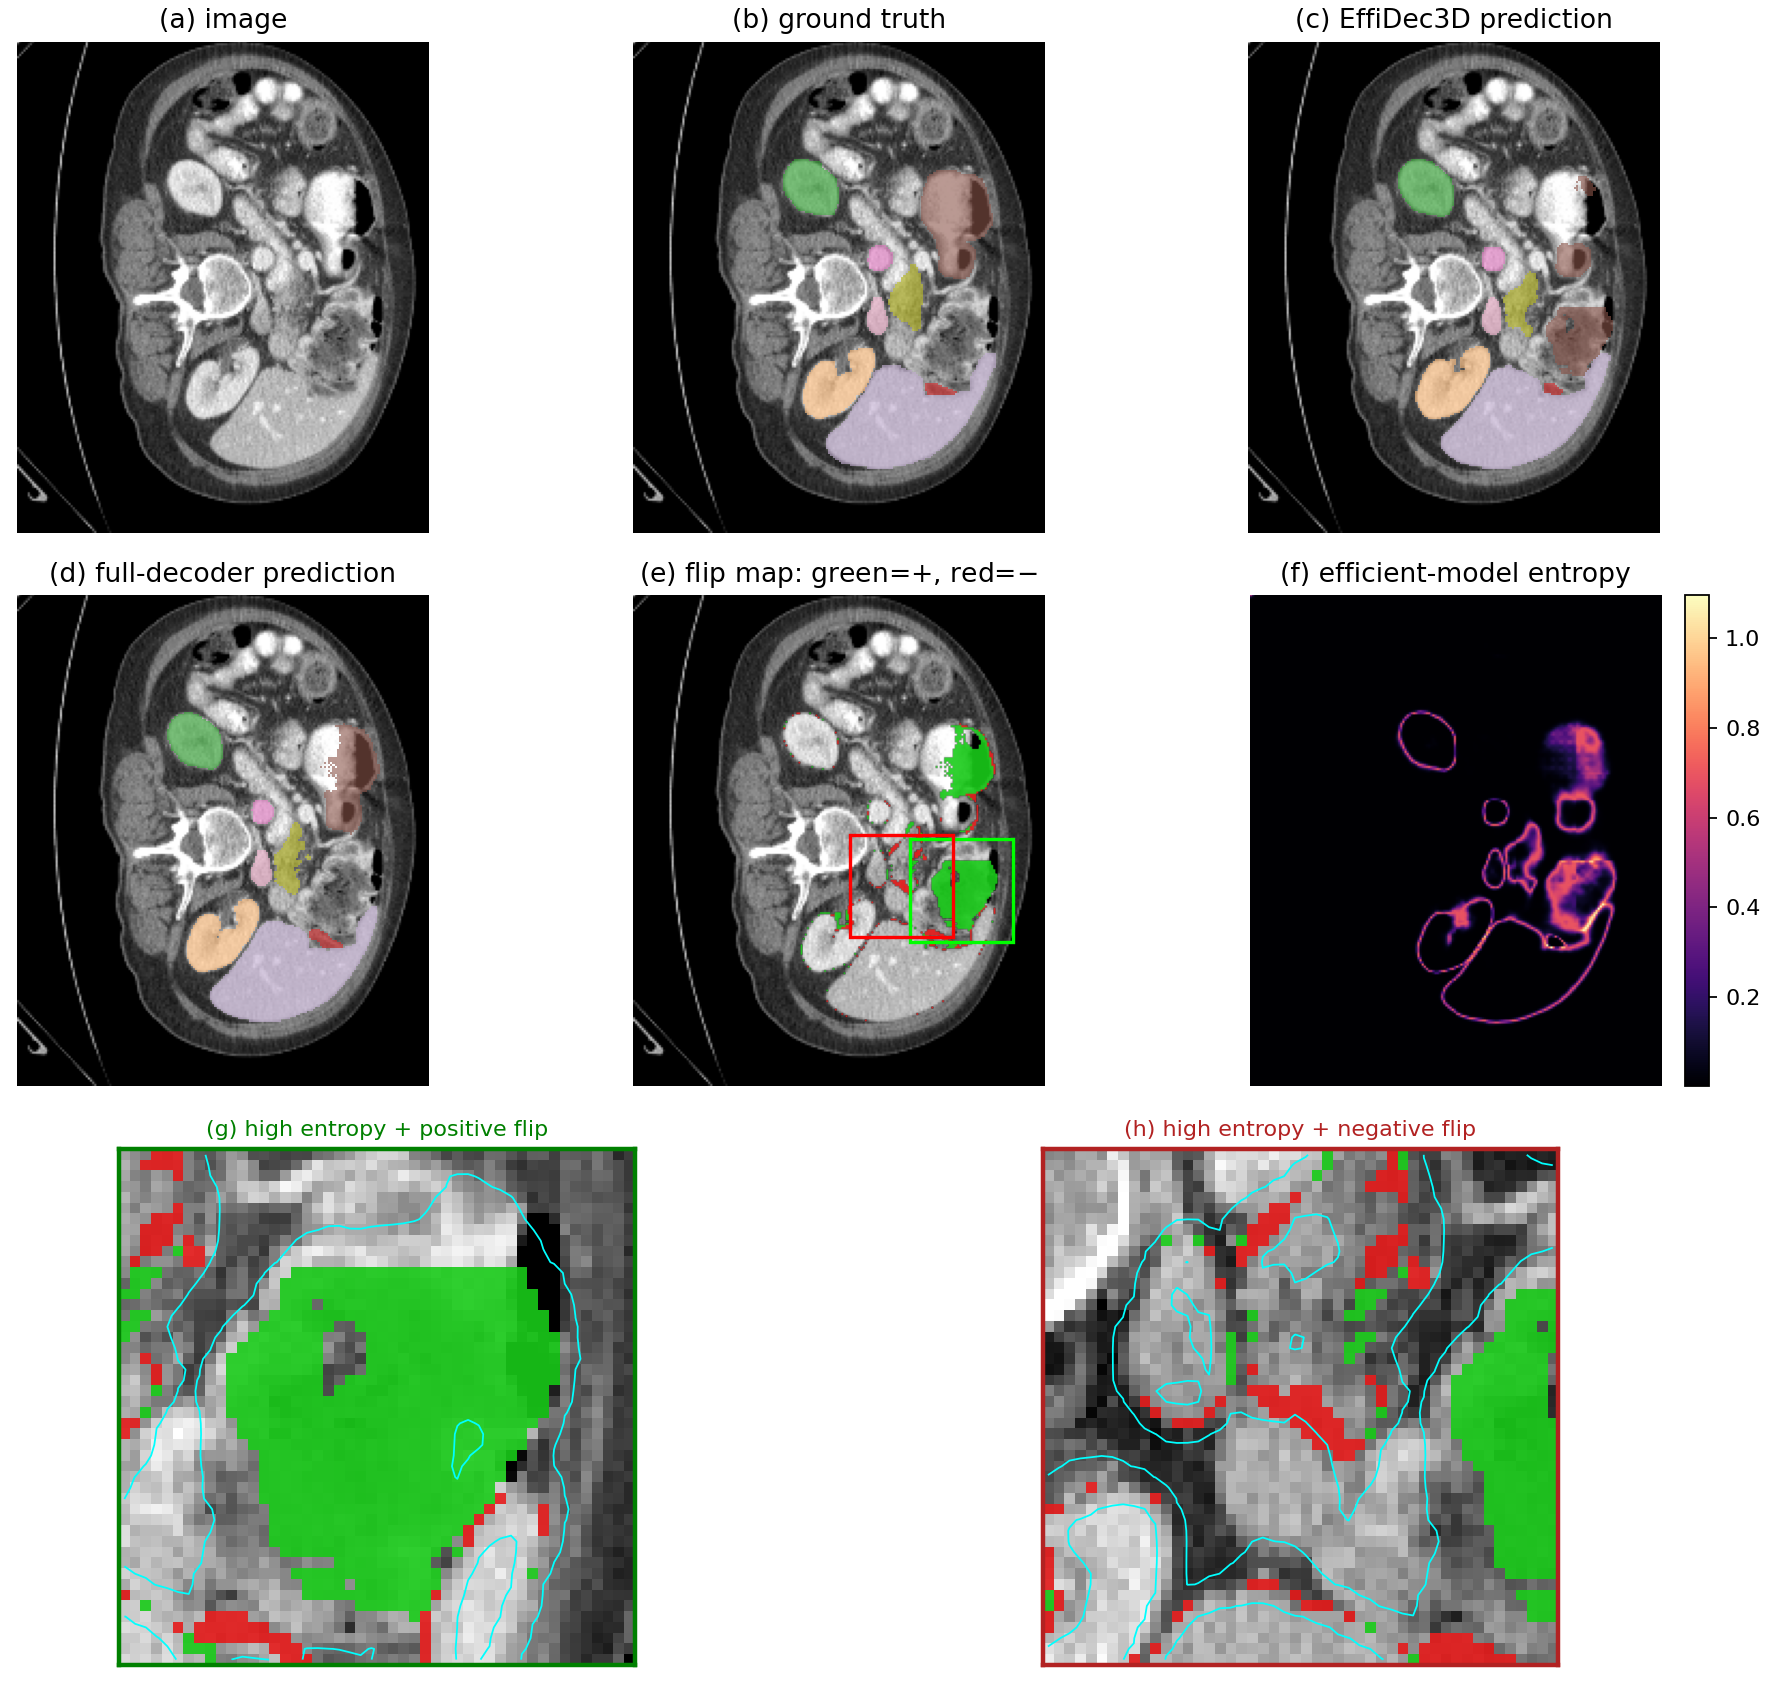
\includegraphics[width=0.95\textwidth]{figures/obs-mednext/figure1_motivation.png}
\caption{Supplementary Figure S2: Qualitative motivation visualization for MedNeXt-M-K3 on BTCV CT multi-organ dataset under Full ($E_0$) vs. Efficient ($E_1$) decoders.}
\label{fig:supp_mednext}
\end{figure*}

\section*{Supplementary Material: Entropy Monotonicity with Block-Level Error Rate}

Figure \ref{fig:supp_error_rate} visualizes the block-level spatial correlation between mean predictive entropy and block-level error rate across all three evaluated backbones. The monotonic relationship confirms that entropy reliably localizes active, error-prone regions (Location AUROC), even though its directional discrimination ability remains weak.

\begin{figure*}[htbp]
\centering
\begin{tabular}{ccc}

\includegraphics[width=0.32\textwidth]{figures/obs-uxnet-concat/O3_unc_error.png} &

\includegraphics[width=0.32\textwidth]{figures/obs-swin-concat/O3_unc_error.png} &

\includegraphics[width=0.32\textwidth]{figures/obs-mednext/O3_unc_error.png} \\
(a) 3D UX-Net Error Correlation & (b) SwinUNETR Error Correlation & (c) MedNeXt-M-K3 Error Correlation \\
\end{tabular}
\caption{Supplementary Figure S3: Correlation between mean predictive entropy and block-level error rate across backbones.}
\label{fig:supp_error_rate}
\end{figure*}

\section*{Supplementary Material: Additional Implementation Details}

\subsection*{TTA-MI (Test-Time Augmentation Mutual Information) Setup}
For evaluating the predictive power of multi-view epistemic disagreement against spatial entropy, we utilized 8-view Test-Time Augmentation (TTA). Each volume was forwarded through the network across all 8 spatial flip combinations ($x, y, z$ axes). The Mutual Information (TTA-MI) was computed as the difference between the entropy of the mean prediction and the mean of the individual view entropies. Despite this computationally expensive multi-pass estimation, TTA-MI provided only marginally better directional discrimination (Direction AUROC 0.570 for SwinUNETR, 0.539 for 3D UX-Net) compared to single-pass predictive entropy, further reinforcing our conclusion that uncertainty measures are powerful activity indicators but weak directional utility classifiers.

\end{document}
